Evaluation of ESN performance on the NARMA system is a thoroughly explored area
in the field of RC \cite{verstraeten_experimental_2007, rodan_minimum_2011,
jaeger_adaptive_nodate}. Similar performance to previous work has been achieved
(Fig. \ref{visualization}, \ref{performance}) as a baseline to lend credibility
to further approaches in this paper.

\begin{figure}[H]
  \centering
  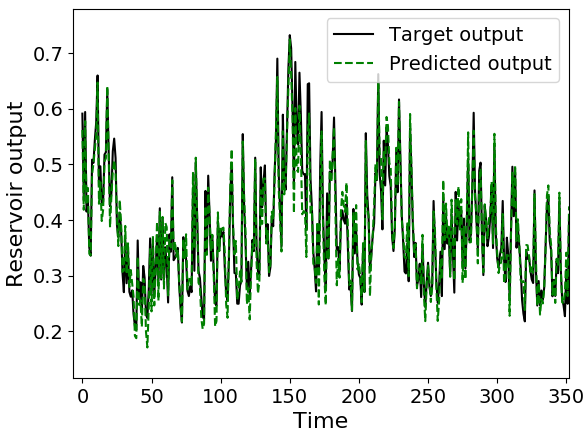
\includegraphics[width=2.5in]{img/narma_visualization.png}
  \caption{
    Visualization of reservoir output when fed the NARMA10 task. Input is an
i.i.d. stream generated uniformly in the interval [0, 0.5].
  }
  \label{visualization}
\end{figure}

\begin{figure}[H]
  \centering
  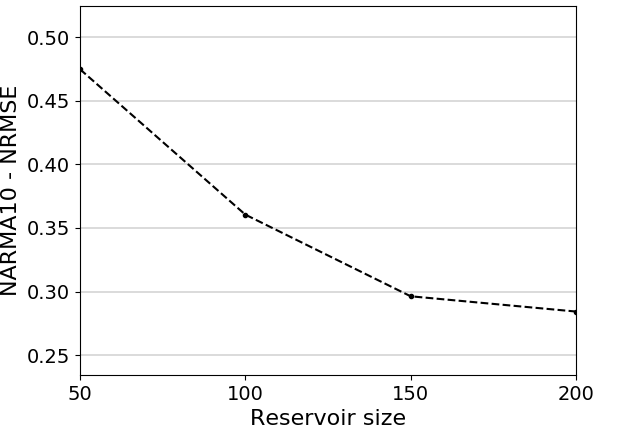
\includegraphics[width=2.5in]{img/general_performance.png}
  \caption{
    Reservoir size versus ESN performance for the NARMA10 task. The NRMSE is
averaged over 10 simulation runs.
  }
  \label{performance}
\end{figure}

All further reservoirs were constructed with the parameters from this baseline:
$\mathbf{W}^{res}$ and $\mathbf{W}^{in}$ were both generated as random matrices
with i.i.d. entries in the interval [-0.5, 0.5]. Both matrices are fully
connected, and the reservoir weight matrix was rescaled to have a spectral
radius of 0.9.

% (TODO): w_res density was also set to 0.2.

% (TODO): The code base is available at <link>.

% (TODO): All experiments are conducted with 10 reservoirs per point.

\subsection{Noise}

Key point: as long as we train with noise, we become more robust.

\begin{figure}[H]
  \centering
  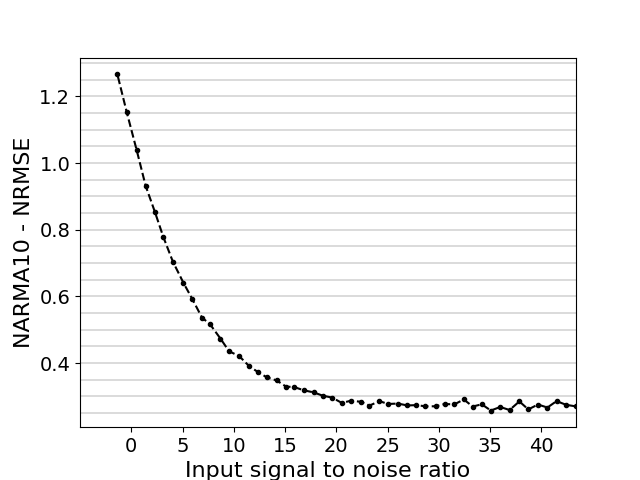
\includegraphics[width=2.5in]{img/input_noise_snr.png}
  \caption{
    Input noise SNR versus NRMSE.
  }
  \label{input_noise_snr}
\end{figure}

Some text.

\begin{figure}[H]
  \centering
  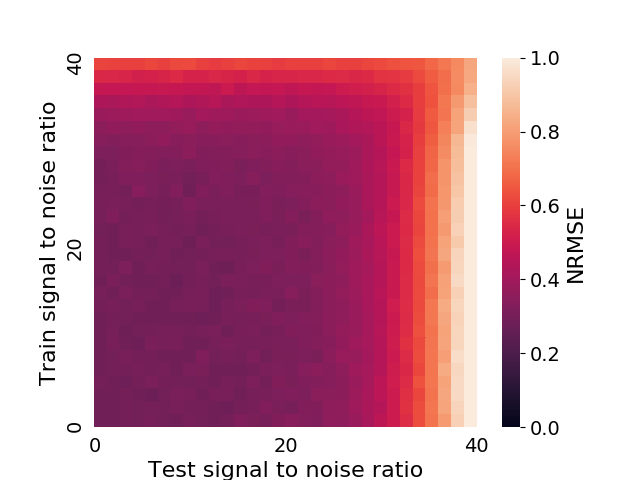
\includegraphics[width=2.5in]{img/input_noise_heatmap.png}
  \caption{
    Input noise signal to noise ratio for test/train.
  }
  \label{input_noise_heatmap}
\end{figure}

More text.

\subsection{Measurement equipment accuracy}

When conducting experiments using physical reservoirs, one will inevitably have
to interact with substrates from software. Whether it be transforming digital
representations of reservoir perturbations to analog signals that cause the
excitation, or the reverse mapping of the analog state of the reservoir into a
digital representation, the accuracy of equipment used for such conversions may
be of critical importance.

Here we investigate the impact of the quantization done by ADC systems. Sensor
anomalies, noise and amplification gain may all impact performance, but as found
in the previous subsection, reservoirs prove to be quite robust to the presence
of such noise patterns. We therefore focus 

\begin{figure}[H]
  \centering
  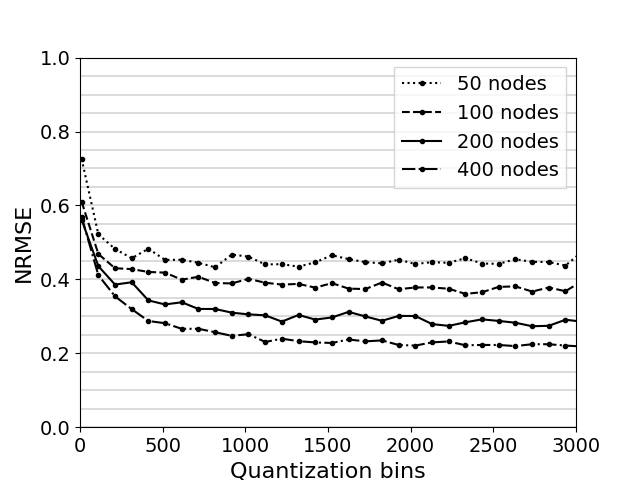
\includegraphics[width=2.5in]{img/adc_quantization.png}
  \caption{
    Performance effect of ADC quantization on four reservoirs of different
sizes. $\tanh$ is used as activation function for the experiment, dividing its
range of (1-, 1) into $n$ discrete output bins.
  }
  \label{adc_quantization}
\end{figure}

To emulate the behavior of an ADC, we extend our ESN model to allow for
quantization of reservoir output before it is passed to the readout layer. This
quantization effectively divides the range of the nonlinear activation function
of each hidden node into a discrete set of fixed output bins.

Fig. \ref{adc_quantization} shows how quantization affects reservoir
performance. We plot the error of four different reservoir sizes: 50, 100, 200
and 400 hidden nodes.

We see a performance degradation from 3000 to 1000 discernible states, something
that is more pressing for the bigger reservoirs. As the amount of discrete
states move beneath 1000, the performance quickly deteriorates, but perhaps not
to the extent that one would expect from dividing the output range of the
reservoir into only 10 bins.

% (TODO): a reservoir of size 400 is as good as one of 50 without quantization at
% just n quantization bins; an interesting result that shows that even with very
% few bins, it is still possible to do the NARMA10 task.

% (TODO): what is a standard quantization for a 12-bit ADC for example? Of course
% depends on voltages and such, but make some assumptions that really drive home
% the fact that it doesn't matter at all.

% (TODO): Perhaps widen the plot to include up to 4000?

% (TODO): Remember that the main point is connections to physical reservoir
% computing, not ESNs in particular (which may also be interesting, however..).

\subsection{Partially visible state}

\begin{figure}[H]
  \centering
  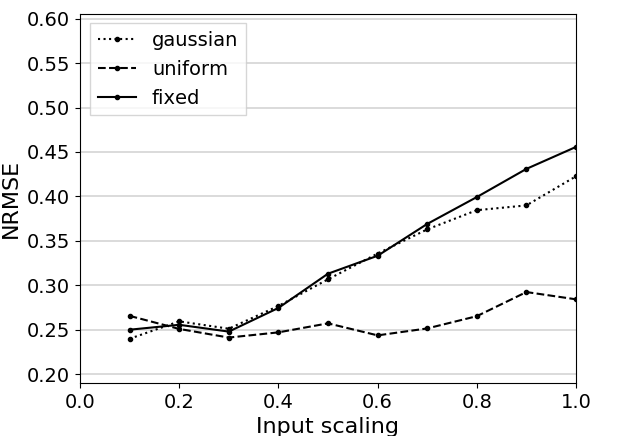
\includegraphics[width=2.5in]{img/input_scaling_distrib.png}
  \caption{
    Effect of input scaling on three input weight distributions.
  }
  \label{input_scaling_distrib}
\end{figure}

\begin{figure*}[htbp]
  \centering
  \begin{subfigure}{.3\textwidth}
    \centering
    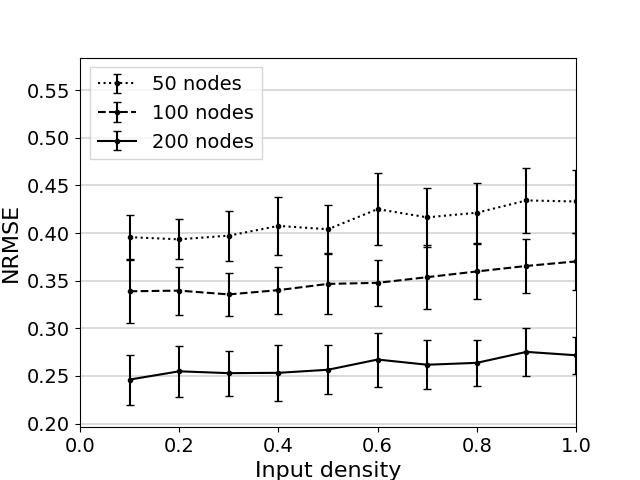
\includegraphics[width=\linewidth]{img/input_density_all.png}
  \end{subfigure}
  \begin{subfigure}{.3\textwidth}
    \centering
    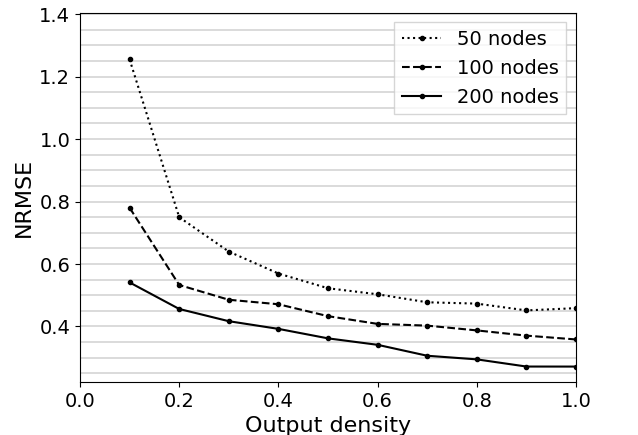
\includegraphics[width=\linewidth]{img/output_density_all.png}
  \end{subfigure}
  \begin{subfigure}{.3\textwidth}
    \centering
    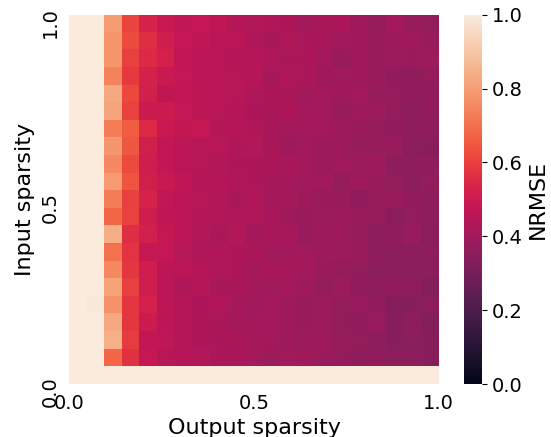
\includegraphics[width=\linewidth]{img/partial_visibility.png}
  \end{subfigure}
  \caption{
    These figures show the influence of reservoirs that are only partially
visible on the performance for the NARMA10 task. Experiments for the rightmost
plot were conducted using a reservoir size of 200 hidden nodes. The density is a
measurement for the fraction of elements in the input and output matrices
containing non-zero elements.
  }
  \label{partial_visibility}
\end{figure*}

% (TODO): Tie this together with topology, if it has a feed-forward-like structure
% or similar.

\subsection{Topology}

\begin{figure}[H]
  \centering
  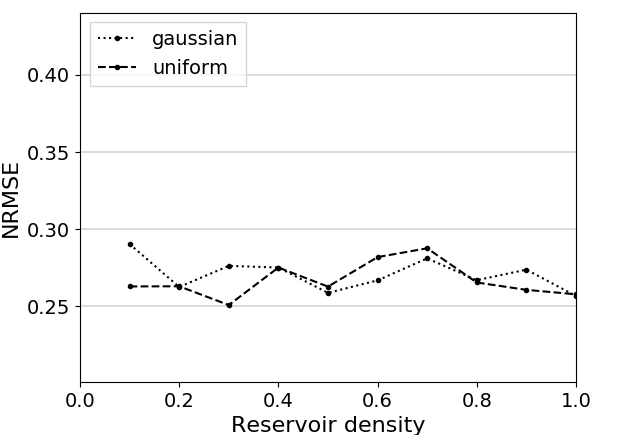
\includegraphics[width=2.5in]{img/reservoir_density_distrib.png}
  \caption{
    Reservoir density versus for two weight distributions. Fixed weight will not
work for internal nodes, unless special topology is employed, e.g. ring
(elaborate). This shows that sparse internal weight matrices work fine.
  }
  \label{reservoir_density_distrib}
\end{figure}

% (TODO): Is w_density also interesting for physical reservoirs?

%%% Local Variables:
%%% mode: latex
%%% TeX-master: "../main"
%%% End:
